\documentclass[12pt,fleqn]{article}\usepackage{../common}
\begin{document}
Ders 7

Bug�n pozitif kesinlik (positive definite) g�n�. Simdiye kadar lineer
cebirin temellerini isledik, bundan sonra uygulamalara daha agirlik
verecegiz, tabii ki matrisler yapacagimiz her seyin temelinde olmaya devam
edecekler. Konuya su acilardan yaklasacagiz:

* Testler

* Anlam

* Uygulamalar

Ilk once testler. Pozitif kesinlik kelimesi soyleyince matrisin simetrik
oldugunu anlamak gerekiyor, yani matrisin reel ozdegerleri var, ve pek cok
diger ozelligi de var muhakkak, mesela ozvektorlerinin birbirine dik olmasi
gibi. Bu derste daha fazla ozellik gorecegiz, ve bu ekstralar ozellikler
uygulamalarda hakikaten muthis faydalar sagliyorlar.

Daha once soyledigimiz gibi pozitif kesinlik lineer cebirin tamamini bir
araya getirir. Testleri sunlardir:

1. Tum pivotlar $>$ 0 

2. Tum usts sol determinantlar (upper left determinants)  $>$ 0

3. Tum ozdegerler $>$ 0

``Ust sol'' ile neyi kastediyorum? 3x3 bir matriste (alttaki resim) kareye
alinilmis bolumlerden. Bunlardan birincisi sadece $a$ degerini
veriyor. Ikinci ust sol determinant $ac - b^2$ (iki tane $b$ var cunku
matris simetrik, unutmayalim) degerini veriyor, vs. Bu iki degerin de
sifirdan buyuk olmasi gerekiyor. Tabii ki ana determinantin da $>$ 0 olmasi
gerekiyor. Dogal olarak $ac > b^2$, caprazdaki carpim, capraz disindaki
degerlerin carpimini ``pozitiflikte gecmeli'', baska turlu cikarma islemi
pozitif sonuc vermezdi.

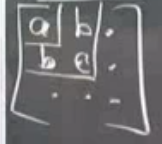
\includegraphics[height=2cm]{7_1.png}

Anlama gelelim. Pozitif kesinlik kavrami, bir egrinin [eliyle konveks bir
parabol hareketi yapiyor, onun alt noktasini kastederek] minimumunu bulmak
ile yakindan alakali, ya da ``enerjiyi azaltma'' problemleriyle alakali. Bu
fiziksel anlami bu ozelligin uygulamalarda niye bu kadar faydali olmasinin
da bir sebebi aslinda. $x$'in bir fonksiyonunu hayal edelim:

\[ f(x) = x^TKx \]

ve diyelim ki $K$

\[ 
\left[\begin{array}{rr}
a & b \\
b & c
\end{array}\right]
 \]

bu derste $x$'in kendisi ile carpimini ilk kez kullaniyoruz bu arada. Bu
form dogal olarak karesel bir sonuc ortaya cikartacak. Biraraya koyarsak

\[ f(x) =
\left[\begin{array}{rr}
x_1 & x_2 
\end{array}\right]
\left[\begin{array}{rr}
a & b \\
b & c
\end{array}\right]
\left[\begin{array}{r}
x_1 \\ x_2 
\end{array}\right]
 \]

Sonuc hangi boyutlarda cikar?

\[ f(x) = \underbrace{x}_{1xn}^T\underbrace{K}_{nxn}\underbrace{x}_{nx1} \]

Zinciri takip edersek, 1x1 boyutlarinda. Temel lineer cebirden hatirlarsak,
NxM ve MxK carpimi NxK boyutlarinda bir matris cikartir. Elde edecegimiz
1x1 ise, bu tek bir sayidir. Tek sayinin bilesenleri nedir? Carpimi
cebirsel olarak takip edersek

\[ = ax_1^2 + 2bx_1x_2 + cx_2^2 \]

Iste ``enerji'' formulu bu, bu forma niye enerji dedigimiz ileriki
derslerde uygulamalara girince daha da iyi belli olacak. Formun cok onemli
bir anlami var. 

Bu noktada ustte belirttigim testlere bir 4. kalem ekleyebilirim, hatta
onemini belirtmek icin basina yildiz bile koymak dusunulebilir!

4. $x=0$ haricindeki tum $x$'ler icin $x^TKx > 0$. 

Bu son formulu aciklamak icin bir grafik cizelim. 

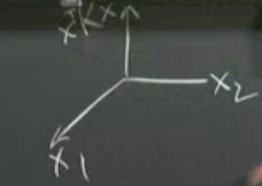
\includegraphics[height=2cm]{7_2.png}

Degisen her $x_1$ ve $x_2$'ya gore hesaplanan, cizilen $x^TKx$'in grafigi
yani. Bu grafik neye benzerdi acaba? Sifirdan baslarsam hep yukari gider
degil mi? Bir kapa benzerdi, ve resmi asagi yukari soyle olurdu. 

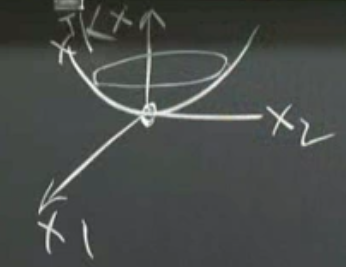
\includegraphics[height=2cm]{7_3.png}

$K$ yerine diger bazi pozitif kesin matrisleri dusunelim. Mesela birim
matris hangi $f(x)$'e sebep olur? $x_1^2 + x_2^2$, ki bu formulde mukemmel
bir kap seklini ortaya cikartir. Ya su matris olsaydi?

\[ 
\left[\begin{array}{rr}
1 & 2 \\
2 & 9
\end{array}\right]
 \]

Sonuc $x_1^2 + 4x_1x_2 + 9x_2^2$ olurdu, o zaman sekil ust kesitinde daha
eliptik bir sekilde olurdu. Ustteki matriste 2 degerinden yukari
cikabiliriz, ama pozitif kesinlik istiyorsak bu $9 \cdot 1$'i gecmeyecak
kadar olmali.

Ilginc bir durum pozitif kesinligin tan s�n�r�ndaki durumdur. Matematikte
bu t�r s�n�r sartlar� anlamak butunu kavramakta faydali oluyor. Mesela
ustteki ornekte 2 yerine 3 olsaydi o zaman

\[ 
\left[\begin{array}{rr}
1 & 3 \\
3 & 9
\end{array}\right]
 \]

Bu matrise bakalim, ikinci kolon birincisinin ``kat�'' oldugu icin hemen
bu matrisin tekil oldugunu anliyoruz. O zaman ozdegerlerinden biri
kesinlikle 0 olmali. Matrisi izi ozdeger toplamini verdigine gore ikinci
ozdeger 10. Formulu neye benzer? $x_1^2 + 6x_1x_2 + 9x_2^2$. Bu tur
matrislere pozitif yari-kesin (semi-definite) deniyor. Ozdegerleri $\ge 0$,
determinantlari $\ge 0$, ve sebep olduklar� $f(x) \ge 0$, yani enerjileri
$\ge 0$. 

Mantik yurutmeye devam edelim. Pozitif yari kesinlik tekil bir matrisin
oldugu anlamina geliyorsa, o zaman bazi $x$ degerleri icin $f(x)$ sifir
olacak demektir. Ustteki ornekte bu hangi deger? [3 -1]'i deneyelim, ve
carpimi yapalim

\[ 
\left[\begin{array}{rr}
1 & 3 \\
3 & 9
\end{array}\right]
\left[\begin{array}{r}
3 \\
-1
\end{array}\right] =
\left[\begin{array}{r}
0 \\
0
\end{array}\right] 
 \]

Hakikaten de $x_1 = 3$ ve $x_2=-1$ kullaninca $x_1^2 + 6x_1x_2 + 9x_2^2$
formulunun sifir sonucunu verdigini goruruz. Sekil asagi yukari soyle:

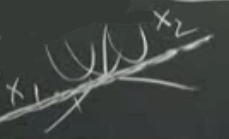
\includegraphics[height=2cm]{7_4.png}

Hoca bu sekli cizmek icin $x_1$ uzerinde 3 birim ileri, $x_2$ uzerinde 1
birim geri gitti, ve o noktadan gecen bir cizgi uzerinde degisim, yukari
asagi gidis yok. Bu cizgi tabii ki 3 ve -1'in katlari alinarak elde
edilebilecek noktalardan olusuyor, ve bu noktalar ustteki matrisin
``sifirlik uzayinda (nullspace)''. Pozitif kesin matrislerden gelen
grafikler, kiyasla, boyle degildi. O grafiklerde kap uzerindeki her
noktadaki gidis yonu yukari isaret ediyordu.

Daha iyi cizilmis bir sekil soyle:

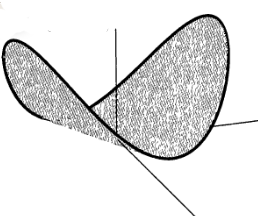
\includegraphics[height=2cm]{7_5.png}

Simdi de pozitif yari-kesin bile olmayan bir matrisi dusunelim. Bu matriste
capraz disi (off-diagonal) degerler cok daha buyuk ve ``kazaniyorlar''. Ornek

\[ 
\left[\begin{array}{rr}
x_1 & x_2 
\end{array}\right]
\left[\begin{array}{rr}
1 & 5 \\
5 & 9
\end{array}\right]
\left[\begin{array}{r}
x_1 \\ x_2 
\end{array}\right] =
x_1^2 + 10x_1x_2 + 9x_2^2
 \]

Bu formulu belli bazi $x$ degerleriyle negatif yapmak mumkun. Hangi
degerler mesela? Diyelim ki $x_1 = -1$ ve $x_2 = 1/2$. Bu formul bazi
noktalarda asagi, bazilarinda yukari gidebiliyor. Bu durumu ortaya cikartan
matrislere ``tanimsiz (indefinite)'' ismi veriliyor. Grafigi alttaki gibi,
atlarin uzerine koyulan bir eger gibi. 

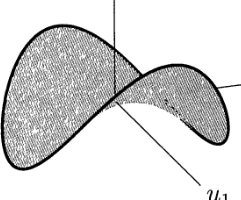
\includegraphics[height=2cm]{7_6.png}

Bunlar onemli noktalar. Simdi biraz ileri atlayalim. Elimizde bazi
secenekler var. Mesela tipik olarak $Ku = f$ durumunda bir formul
cozuyorduk ve tek bir cozum buluyorduk. Bir diger secenek te bir
fonksiyonu, bir enerjiyi minimize etmek. Uygulamalar icin secenekler
bunlar. 

Pozitif kesin matrisler alttaki ifadeden gelirler. Bu kavram test olarak ta
anlamli, o yuzden testlere bir 5. kalem ekleyecegiz. 

5. $K = A^TA$. 

Bu ifade pozitif kesin. Niye? $x^TKx = x^TA^TAx$'ye bakalim.

\[ x^TA^TAx \]

Bu ifade aslinda su degil mi?

\[ = (Ax)^T(Ax) \]

Ve bu ifadenin de $(Ax)^T(Ax) \ge 0$ oldugunu biliyoruz, cunku $Ax$'in
devrigi tekrar kendisi ile carpiliyor. Ifadenin sifira esit olmasi ancak
$Ax=0$ ise mumkundur. Mantik zincirine devam edersek, $Ax=0$'yi cozen bir
$x$ varsa ($A$'nin sifir uzayi bos degilse), yani $Ax=0$'e sebep olacak
sifir vektoru haricinde bir $x$ mevcutsa, o zaman $(Ax)^T(Ax)$ pozitif
yari-kesin demektir, cunku o zaman $Ax=0$ olabilecektir. 

$Ax=0$ uygulamalarda nasil ortaya cikar? Mesela bir yay sisteminde eger yer
degisimi var ama yay esnemesi yoksa ($Ax$ yay esnemesini olcer), bu durum
ortaya cikabilir. Peki bu nasil mumkun olabilir, yay esnemeden, daralmadan
nasil hareket olabilir?  Eger yay sistemini ``tamami'' kaldirilip baska
yere goturulurse . Bu sistem serbest-serbest sistemi ile mumkun, yani iki
ucum bir yere bagli olmadigi bir yay sisteminde, sistem [1 1 1] vektoru ile
bir yere tasiniyor. Bu durumda matris tekil demektir, cunku pozitif
yari-kesindir. Yani tipik matrislerimizden

$K,T$ pozitif kesin. 

$B, C$ pozitif yari-kesin. 

Mantiga devam: Sadece ve sadece $A$ matrisinin bagimsiz kolonlari var ise,
o zaman $Ax$ pozitif kesindir. 

Simdi pozitif-kesin matrislerin tersini (inverse) dusunelim. Tersini alinca
ele gecen matris te pozitif kesin midir? Bunu kararlastirmak icin elimizde
bir suru test var. Pivot ve determinantlara girmek biraz isleri karistirir,
ama ozdegerlere ne olur, kendimize bunu soralim. Bu ozdegerlerin ne
olacagini hemen biliyoruz, mesela elimizde 3,4,5 gibi ozdegerler olsa
(hepsi pozitif tabii ki), matrisin tersini alinca elde edecegimiz
ozdegerler 1/3,1/4,1/5 gibi degerler olacaktir, ki bu degerler de
pozitiften. 1'den kucuk olabilirler ama 0'dan buyukturler. En basit kontrol
edilebilecek test buydu. Pozitif kesinlik icin butun testlerin dogru olmasi
gerekir. 

Peki elimizde iki pozitif kesin matris $K_1$ ve $K_2$ varsa 

\[ K_1 + K_2 \]

pozitif kesin midir? Bu toplamin ozdegerlerine bakmak zor olur. Fakat
4. testi kullanabiliriz. $K_1$ ve $K_2$'yi $x$ ile carpalim. 

\[ x^TK_1x + x^TK_2x \]

Formuldeki her terim sifirdan buyuktur, cunku bu pozitif kesinligin
tanimi. O zaman toplam da sifirdan buyuk olacaktir. Bu sonuca eristikten
sonra, simdi cebirsel olarak basitlestiririz:

\[ x^T(K_1 + K_2)x \]

Ve iki pozitif kesin matrisin toplamina erismis oluruz. Demek ki iki
pozitif kesin matrisin toplami da pozitif kesindir. 

Peki toplam soyle olsaydi?

\[ \underbrace{K_1}_{A^TA} + \underbrace{K_2}_{B^TB} \]

A ve B'yi tek bir matris icine koydugumuzu varsayalim, ki bu matrislere
``blok matrisleri'' deniyor:

\[ C = 
\left[\begin{array}{r}
A \\
B
\end{array}\right]
 \]

Blok matrisinin devrigi nedir? 

\[ 
C^T = 
\left[\begin{array}{rr}
A^T & B^T
\end{array}\right]
 \]

Blok matrisleri nasil carparim?

\[ 
C^TC = A^TA + B^TB 
 \]

Bu $K_1 + K_2$'ya esittir. 

\end{document}
